\documentclass[twoside]{book}

% Packages required by doxygen
\usepackage{calc}
\usepackage{doxygen}
\usepackage{graphicx}
\usepackage[utf8]{inputenc}
\usepackage{makeidx}
\usepackage{multicol}
\usepackage{multirow}
\usepackage{textcomp}
\usepackage[table]{xcolor}

% Font selection
\usepackage[T1]{fontenc}
\usepackage{mathptmx}
\usepackage[scaled=.90]{helvet}
\usepackage{courier}
\usepackage{amssymb}
\usepackage{sectsty}
\renewcommand{\familydefault}{\sfdefault}
\allsectionsfont{%
  \fontseries{bc}\selectfont%
  \color{darkgray}%
}
\renewcommand{\DoxyLabelFont}{%
  \fontseries{bc}\selectfont%
  \color{darkgray}%
}

% Page & text layout
\usepackage{geometry}
\geometry{%
  a4paper,%
  top=2.5cm,%
  bottom=2.5cm,%
  left=2.5cm,%
  right=2.5cm%
}
\tolerance=750
\hfuzz=15pt
\hbadness=750
\setlength{\emergencystretch}{15pt}
\setlength{\parindent}{0cm}
\setlength{\parskip}{0.2cm}
\makeatletter
\renewcommand{\paragraph}{%
  \@startsection{paragraph}{4}{0ex}{-1.0ex}{1.0ex}{%
    \normalfont\normalsize\bfseries\SS@parafont%
  }%
}
\renewcommand{\subparagraph}{%
  \@startsection{subparagraph}{5}{0ex}{-1.0ex}{1.0ex}{%
    \normalfont\normalsize\bfseries\SS@subparafont%
  }%
}
\makeatother

% Headers & footers
\usepackage{fancyhdr}
\pagestyle{fancyplain}
\fancyhead[LE]{\fancyplain{}{\bfseries\thepage}}
\fancyhead[CE]{\fancyplain{}{}}
\fancyhead[RE]{\fancyplain{}{\bfseries\leftmark}}
\fancyhead[LO]{\fancyplain{}{\bfseries\rightmark}}
\fancyhead[CO]{\fancyplain{}{}}
\fancyhead[RO]{\fancyplain{}{\bfseries\thepage}}
\fancyfoot[LE]{\fancyplain{}{}}
\fancyfoot[CE]{\fancyplain{}{}}
\fancyfoot[RE]{\fancyplain{}{\bfseries\scriptsize Generated on Tue Jun 15 2021 15\-:01\-:35 for Tool\-Framework\-Application by Doxygen }}
\fancyfoot[LO]{\fancyplain{}{\bfseries\scriptsize Generated on Tue Jun 15 2021 15\-:01\-:35 for Tool\-Framework\-Application by Doxygen }}
\fancyfoot[CO]{\fancyplain{}{}}
\fancyfoot[RO]{\fancyplain{}{}}
\renewcommand{\footrulewidth}{0.4pt}
\renewcommand{\chaptermark}[1]{%
  \markboth{#1}{}%
}
\renewcommand{\sectionmark}[1]{%
  \markright{\thesection\ #1}%
}

% Indices & bibliography
\usepackage{natbib}
\usepackage[titles]{tocloft}
\setcounter{tocdepth}{3}
\setcounter{secnumdepth}{5}
\makeindex

% Hyperlinks (required, but should be loaded last)
\usepackage{ifpdf}
\ifpdf
  \usepackage[pdftex,pagebackref=true]{hyperref}
\else
  \usepackage[ps2pdf,pagebackref=true]{hyperref}
\fi
\hypersetup{%
  colorlinks=true,%
  linkcolor=blue,%
  citecolor=blue,%
  unicode%
}

% Custom commands
\newcommand{\clearemptydoublepage}{%
  \newpage{\pagestyle{empty}\cleardoublepage}%
}


%===== C O N T E N T S =====

\begin{document}

% Titlepage & ToC
\hypersetup{pageanchor=false}
\pagenumbering{roman}
\begin{titlepage}
\vspace*{7cm}
\begin{center}%
{\Large Tool\-Framework\-Application }\\
\vspace*{1cm}
{\large Generated by Doxygen 1.8.5}\\
\vspace*{0.5cm}
{\small Tue Jun 15 2021 15:01:35}\\
\end{center}
\end{titlepage}
\clearemptydoublepage
\tableofcontents
\clearemptydoublepage
\pagenumbering{arabic}
\hypersetup{pageanchor=true}

%--- Begin generated contents ---
\chapter{Dummy Tool R\-E\-A\-D\-M\-E}
\label{md_UserTools_DummyTool_README}
\hypertarget{md_UserTools_DummyTool_README}{}
\subsection*{Data}

This Tool Is just a dummy that prints out differnt messges to the consol depending on the debug level.

\subsection*{Configuration}

Describe any configuration variables for \hyperlink{classMyTool}{My\-Tool}.

verbose value \# any int for the value 
\chapter{D\-A\-Q\-Framework}
\label{md_UserTools_InactiveTools_README}
\hypertarget{md_UserTools_InactiveTools_README}{}
\input{md_UserTools_InactiveTools_README}
\chapter{D\-A\-Q\-Framework}
\label{md_UserTools_README}
\hypertarget{md_UserTools_README}{}
\input{md_UserTools_README}
\chapter{D\-A\-Q\-Framework}
\label{md_UserTools_template_README}
\hypertarget{md_UserTools_template_README}{}
\input{md_UserTools_template_README}
\chapter{R\-E\-A\-D\-M\-E}
\label{md_DataModel_README}
\hypertarget{md_DataModel_README}{}
\#\+Data Model \DoxyHorRuler{0}


Data Model Class can be defined how ever the User requires. A Store is provided which ineficently maps variables to string lkeys via conversion to stringstream and can be used for debuging or other useful vairables.

A TTree map with getter and setter functions is provided and can be uncommented if required. 
\chapter{Hierarchical Index}
\doxysection{Class Hierarchy}
This inheritance list is sorted roughly, but not completely, alphabetically\+:\begin{DoxyCompactList}
\item \contentsline{section}{CAMAC\+\_\+args\+\_\+args}{\pageref{structCAMAC__args__args}}{}
\item \contentsline{section}{Camac\+Crate}{\pageref{classCamacCrate}}{}
\begin{DoxyCompactList}
\item \contentsline{section}{Le\+Croy4413}{\pageref{classLeCroy4413}}{}
\item \contentsline{section}{Lecroy3377}{\pageref{classLecroy3377}}{}
\item \contentsline{section}{Lecroy4300b}{\pageref{classLecroy4300b}}{}
\end{DoxyCompactList}
\item \contentsline{section}{MRDData\+::Card}{\pageref{structMRDData_1_1Card}}{}
\item \contentsline{section}{MRDData\+::Channel}{\pageref{structMRDData_1_1Channel}}{}
\item \contentsline{section}{Data\+Model}{\pageref{classDataModel}}{}
\item \contentsline{section}{Data\+Model\+Thread\+\_\+args}{\pageref{structDataModelThread__args}}{}
\item \contentsline{section}{JSONP}{\pageref{classJSONP}}{}
\item \contentsline{section}{Json\+Parser\+Result}{\pageref{structJsonParserResult}}{}
\item \contentsline{section}{LAPPD\+\_\+args\+\_\+args}{\pageref{structLAPPD__args__args}}{}
\item \contentsline{section}{MRDData\+::Module}{\pageref{structMRDData_1_1Module}}{}
\item \contentsline{section}{MRDData}{\pageref{classMRDData}}{}
\item \contentsline{section}{My\+Tool\+Thread\+\_\+args\+\_\+args}{\pageref{structMyToolThread__args__args}}{}
\item \contentsline{section}{PGClient}{\pageref{classPGClient}}{}
\item \contentsline{section}{PGHelper}{\pageref{classPGHelper}}{}
\item \contentsline{section}{Psec\+Data}{\pageref{classPsecData}}{}
\item \contentsline{section}{Query}{\pageref{structQuery}}{}
\item \contentsline{section}{Serialisable\+Object}{\pageref{classSerialisableObject}}{}
\begin{DoxyCompactList}
\item \contentsline{section}{Card\+Data}{\pageref{classCardData}}{}
\item \contentsline{section}{MRDOut}{\pageref{classMRDOut}}{}
\item \contentsline{section}{Trigger\+Data}{\pageref{classTriggerData}}{}
\end{DoxyCompactList}
\item \contentsline{section}{Store\+Save\+\_\+args\+\_\+args}{\pageref{structStoreSave__args__args}}{}
\item \contentsline{section}{Thread\+\_\+args}{\pageref{structThread__args}}{}
\begin{DoxyCompactList}
\item \contentsline{section}{CAMAC\+\_\+args}{\pageref{structCAMAC__args}}{}
\item \contentsline{section}{DAQThread\+\_\+args}{\pageref{structDAQThread__args}}{}
\begin{DoxyCompactList}
\item \contentsline{section}{LAPPD\+\_\+args}{\pageref{structLAPPD__args}}{}
\item \contentsline{section}{My\+Tool\+ZMQMulti\+Thread\+\_\+args}{\pageref{structMyToolZMQMultiThread__args}}{}
\item \contentsline{section}{VME\+\_\+args}{\pageref{structVME__args}}{}
\end{DoxyCompactList}
\item \contentsline{section}{My\+Tool\+Dynamic\+Multi\+Thread\+\_\+args}{\pageref{structMyToolDynamicMultiThread__args}}{}
\item \contentsline{section}{My\+Tool\+Multi\+Thread\+\_\+args}{\pageref{structMyToolMultiThread__args}}{}
\item \contentsline{section}{My\+Tool\+Thread\+\_\+args}{\pageref{structMyToolThread__args}}{}
\item \contentsline{section}{Store\+Save\+\_\+args}{\pageref{structStoreSave__args}}{}
\end{DoxyCompactList}
\item Tool\begin{DoxyCompactList}
\item \contentsline{section}{CAMAC}{\pageref{classCAMAC}}{}
\item \contentsline{section}{Dummy\+Tool}{\pageref{classDummyTool}}{}
\item \contentsline{section}{LAPPD}{\pageref{classLAPPD}}{}
\item \contentsline{section}{My\+Tool}{\pageref{classMyTool}}{}
\item \contentsline{section}{My\+Tool\+Dynamic\+Multi\+Thread}{\pageref{classMyToolDynamicMultiThread}}{}
\item \contentsline{section}{My\+Tool\+Multi\+Thread}{\pageref{classMyToolMultiThread}}{}
\item \contentsline{section}{My\+Tool\+Service\+Add}{\pageref{classMyToolServiceAdd}}{}
\item \contentsline{section}{My\+Tool\+Thread}{\pageref{classMyToolThread}}{}
\item \contentsline{section}{My\+Tool\+ZMQMulti\+Thread}{\pageref{classMyToolZMQMultiThread}}{}
\item \contentsline{section}{PGStarter}{\pageref{classPGStarter}}{}
\item \contentsline{section}{Run\+Control}{\pageref{classRunControl}}{}
\item \contentsline{section}{Slack\+Bot}{\pageref{classSlackBot}}{}
\item \contentsline{section}{Store\+Save}{\pageref{classStoreSave}}{}
\item \contentsline{section}{VME}{\pageref{classVME}}{}
\end{DoxyCompactList}
\item \contentsline{section}{usb\+\_\+bus}{\pageref{structusb__bus}}{}
\item \contentsline{section}{usb\+\_\+config\+\_\+descriptor}{\pageref{structusb__config__descriptor}}{}
\item \contentsline{section}{usb\+\_\+ctrl\+\_\+setup}{\pageref{structusb__ctrl__setup}}{}
\item \contentsline{section}{usb\+\_\+descriptor\+\_\+header}{\pageref{structusb__descriptor__header}}{}
\item \contentsline{section}{usb\+\_\+device}{\pageref{structusb__device}}{}
\item \contentsline{section}{usb\+\_\+device\+\_\+descriptor}{\pageref{structusb__device__descriptor}}{}
\item \contentsline{section}{usb\+\_\+endpoint\+\_\+descriptor}{\pageref{structusb__endpoint__descriptor}}{}
\item \contentsline{section}{usb\+\_\+hid\+\_\+descriptor}{\pageref{structusb__hid__descriptor}}{}
\item \contentsline{section}{usb\+\_\+interface}{\pageref{structusb__interface}}{}
\item \contentsline{section}{usb\+\_\+interface\+\_\+descriptor}{\pageref{structusb__interface__descriptor}}{}
\item \contentsline{section}{usb\+\_\+string\+\_\+descriptor}{\pageref{structusb__string__descriptor}}{}
\item \contentsline{section}{usb\+\_\+version}{\pageref{structusb__version}}{}
\item \contentsline{section}{Utilities}{\pageref{classUtilities}}{}
\begin{DoxyCompactList}
\item \contentsline{section}{DAQUtilities}{\pageref{classDAQUtilities}}{}
\end{DoxyCompactList}
\item \contentsline{section}{VME\+\_\+args\+\_\+args}{\pageref{structVME__args__args}}{}
\item \contentsline{section}{XXUSB\+\_\+\+CC\+\_\+\+COMMAND\+\_\+\+TYPE}{\pageref{structXXUSB__CC__COMMAND__TYPE}}{}
\item \contentsline{section}{xxusb\+\_\+device\+\_\+typ}{\pageref{structxxusb__device__typ}}{}
\item \contentsline{section}{XXUSB\+\_\+\+STACK}{\pageref{structXXUSB__STACK}}{}
\item \contentsline{section}{ZMQMy\+Tool\+Multi\+Thread\+\_\+args}{\pageref{structZMQMyToolMultiThread__args}}{}
\end{DoxyCompactList}

\chapter{Class Index}
\doxysection{Class List}
Here are the classes, structs, unions and interfaces with brief descriptions\+:\begin{DoxyCompactList}
\item\contentsline{section}{\mbox{\hyperlink{classCardData}{Card\+Data}} }{\pageref{classCardData}}{}
\item\contentsline{section}{\mbox{\hyperlink{structDAQThread__args}{DAQThread\+\_\+args}} }{\pageref{structDAQThread__args}}{}
\item\contentsline{section}{\mbox{\hyperlink{classDAQUtilities}{DAQUtilities}} }{\pageref{classDAQUtilities}}{}
\item\contentsline{section}{\mbox{\hyperlink{classDataModel}{Data\+Model}} }{\pageref{classDataModel}}{}
\item\contentsline{section}{\mbox{\hyperlink{structDataModelThread__args}{Data\+Model\+Thread\+\_\+args}} }{\pageref{structDataModelThread__args}}{}
\item\contentsline{section}{\mbox{\hyperlink{classDummyTool}{Dummy\+Tool}} }{\pageref{classDummyTool}}{}
\item\contentsline{section}{\mbox{\hyperlink{structPostgres_1_1ExpandRow}{Postgres\+::\+Expand\+Row$<$ N, T, Ts $>$}} }{\pageref{structPostgres_1_1ExpandRow}}{}
\item\contentsline{section}{\mbox{\hyperlink{structPostgres_1_1ExpandRow_3_011_00_01T_01_4}{Postgres\+::\+Expand\+Row$<$ 1, T $>$}} }{\pageref{structPostgres_1_1ExpandRow_3_011_00_01T_01_4}}{}
\item\contentsline{section}{\mbox{\hyperlink{classMyTool}{My\+Tool}} }{\pageref{classMyTool}}{}
\item\contentsline{section}{\mbox{\hyperlink{classMyToolDynamicMultiThread}{My\+Tool\+Dynamic\+Multi\+Thread}} }{\pageref{classMyToolDynamicMultiThread}}{}
\item\contentsline{section}{\mbox{\hyperlink{structMyToolDynamicMultiThread__args}{My\+Tool\+Dynamic\+Multi\+Thread\+\_\+args}} }{\pageref{structMyToolDynamicMultiThread__args}}{}
\item\contentsline{section}{\mbox{\hyperlink{classMyToolMultiThread}{My\+Tool\+Multi\+Thread}} }{\pageref{classMyToolMultiThread}}{}
\item\contentsline{section}{\mbox{\hyperlink{structMyToolMultiThread__args}{My\+Tool\+Multi\+Thread\+\_\+args}} }{\pageref{structMyToolMultiThread__args}}{}
\item\contentsline{section}{\mbox{\hyperlink{classMyToolServiceAdd}{My\+Tool\+Service\+Add}} }{\pageref{classMyToolServiceAdd}}{}
\item\contentsline{section}{\mbox{\hyperlink{classMyToolThread}{My\+Tool\+Thread}} }{\pageref{classMyToolThread}}{}
\item\contentsline{section}{\mbox{\hyperlink{structMyToolThread__args}{My\+Tool\+Thread\+\_\+args}} }{\pageref{structMyToolThread__args}}{}
\item\contentsline{section}{\mbox{\hyperlink{structMyToolThread__args__args}{My\+Tool\+Thread\+\_\+args\+\_\+args}} }{\pageref{structMyToolThread__args__args}}{}
\item\contentsline{section}{\mbox{\hyperlink{classMyToolZMQMultiThread}{My\+Tool\+ZMQMulti\+Thread}} }{\pageref{classMyToolZMQMultiThread}}{}
\item\contentsline{section}{\mbox{\hyperlink{structMyToolZMQMultiThread__args}{My\+Tool\+ZMQMulti\+Thread\+\_\+args}} }{\pageref{structMyToolZMQMultiThread__args}}{}
\item\contentsline{section}{\mbox{\hyperlink{classPGHelper}{PGHelper}} }{\pageref{classPGHelper}}{}
\item\contentsline{section}{\mbox{\hyperlink{classPGTool}{PGTool}} }{\pageref{classPGTool}}{}
\item\contentsline{section}{\mbox{\hyperlink{classPostgres}{Postgres}} }{\pageref{classPostgres}}{}
\item\contentsline{section}{\mbox{\hyperlink{classSerialisableObject}{Serialisable\+Object}} }{\pageref{classSerialisableObject}}{}
\item\contentsline{section}{\mbox{\hyperlink{structThread__args}{Thread\+\_\+args}} }{\pageref{structThread__args}}{}
\item\contentsline{section}{\mbox{\hyperlink{classTriggerData}{Trigger\+Data}} }{\pageref{classTriggerData}}{}
\item\contentsline{section}{\mbox{\hyperlink{classUtilities}{Utilities}} }{\pageref{classUtilities}}{}
\item\contentsline{section}{\mbox{\hyperlink{classVME}{VME}} }{\pageref{classVME}}{}
\item\contentsline{section}{\mbox{\hyperlink{structVME__args}{VME\+\_\+args}} }{\pageref{structVME__args}}{}
\item\contentsline{section}{\mbox{\hyperlink{structVME__args__args}{VME\+\_\+args\+\_\+args}} }{\pageref{structVME__args__args}}{}
\item\contentsline{section}{\mbox{\hyperlink{structZMQMyToolMultiThread__args}{ZMQMy\+Tool\+Multi\+Thread\+\_\+args}} }{\pageref{structZMQMyToolMultiThread__args}}{}
\end{DoxyCompactList}

\chapter{Class Documentation}
\hypertarget{classDataModel}{}\doxysection{Data\+Model Class Reference}
\label{classDataModel}\index{DataModel@{DataModel}}


{\ttfamily \#include $<$Data\+Model.\+h$>$}

\doxysubsection*{Public Member Functions}
\begin{DoxyCompactItemize}
\item 
\mbox{\Hypertarget{classDataModel_abff03aef2cb531142a35781bb87c3365}\label{classDataModel_abff03aef2cb531142a35781bb87c3365}} 
\mbox{\hyperlink{classDataModel_abff03aef2cb531142a35781bb87c3365}{Data\+Model}} ()
\begin{DoxyCompactList}\small\item\em Simple constructor. \end{DoxyCompactList}\end{DoxyCompactItemize}
\doxysubsection*{Public Attributes}
\begin{DoxyCompactItemize}
\item 
\mbox{\Hypertarget{classDataModel_a4baac5fe364a7a23762d70d2c2216486}\label{classDataModel_a4baac5fe364a7a23762d70d2c2216486}} 
Store \mbox{\hyperlink{classDataModel_a4baac5fe364a7a23762d70d2c2216486}{vars}}
\begin{DoxyCompactList}\small\item\em This Store can be used for any variables. It is an inefficent ascii based storage. \end{DoxyCompactList}\item 
\mbox{\Hypertarget{classDataModel_a878e0d87285f0b3541a3e7116a5f00b6}\label{classDataModel_a878e0d87285f0b3541a3e7116a5f00b6}} 
Boost\+Store \mbox{\hyperlink{classDataModel_a878e0d87285f0b3541a3e7116a5f00b6}{CStore}}
\begin{DoxyCompactList}\small\item\em This is a more efficent binary Boost\+Store that can be used to store a dynamic set of inter Tool variables. \end{DoxyCompactList}\item 
\mbox{\Hypertarget{classDataModel_ad1ffc080c3b263bf3ee382a531321ad4}\label{classDataModel_ad1ffc080c3b263bf3ee382a531321ad4}} 
std\+::map$<$ std\+::string, Boost\+Store $\ast$ $>$ \mbox{\hyperlink{classDataModel_ad1ffc080c3b263bf3ee382a531321ad4}{Stores}}
\begin{DoxyCompactList}\small\item\em This is a map of named Boo\+Store pointers which can be deffined to hold a nammed collection of any tipe of Boost\+Store. It is usefull to store data that needs subdividing into differnt stores. \end{DoxyCompactList}\item 
\mbox{\Hypertarget{classDataModel_aa777da4c632e4659ee5b1447ad513458}\label{classDataModel_aa777da4c632e4659ee5b1447ad513458}} 
Logging $\ast$ \mbox{\hyperlink{classDataModel_aa777da4c632e4659ee5b1447ad513458}{Log}}
\begin{DoxyCompactList}\small\item\em Log class pointer for use in Tools, it can be used to send messages which can have multiple error levels and destination end points. \end{DoxyCompactList}\item 
\mbox{\Hypertarget{classDataModel_a2c6dfd692e50f90e55338970ea7f8d61}\label{classDataModel_a2c6dfd692e50f90e55338970ea7f8d61}} 
zmq\+::context\+\_\+t $\ast$ \mbox{\hyperlink{classDataModel_a2c6dfd692e50f90e55338970ea7f8d61}{context}}
\begin{DoxyCompactList}\small\item\em ZMQ contex used for producing zmq sockets for inter thread, process, or computer communication. \end{DoxyCompactList}\item 
\mbox{\Hypertarget{classDataModel_a45789efe0f97c28151704dd8afc26899}\label{classDataModel_a45789efe0f97c28151704dd8afc26899}} 
\mbox{\hyperlink{classPGClient}{PGClient}} {\bfseries pgclient}
\item 
\mbox{\Hypertarget{classDataModel_a485ff089c9766544af024d7b57f6859e}\label{classDataModel_a485ff089c9766544af024d7b57f6859e}} 
\mbox{\hyperlink{classPGHelper}{PGHelper}} {\bfseries postgres\+\_\+helper}
\item 
\mbox{\Hypertarget{classDataModel_a17a4172f6f412924e4715ad5774009d0}\label{classDataModel_a17a4172f6f412924e4715ad5774009d0}} 
std\+::vector$<$ std\+::string $>$ {\bfseries identities}
\item 
\mbox{\Hypertarget{classDataModel_a15ae921fea93d47f0096ff27a8810bc2}\label{classDataModel_a15ae921fea93d47f0096ff27a8810bc2}} 
std\+::map$<$ std\+::string, unsigned long $>$ {\bfseries triggers}
\item 
\mbox{\Hypertarget{classDataModel_a89c3baf4a78c1d34019e0ab18f7dfae8}\label{classDataModel_a89c3baf4a78c1d34019e0ab18f7dfae8}} 
unsigned long {\bfseries run}
\item 
\mbox{\Hypertarget{classDataModel_a440fb9bdbac6231aa43c08f044f1fca3}\label{classDataModel_a440fb9bdbac6231aa43c08f044f1fca3}} 
unsigned long {\bfseries subrun}
\item 
\mbox{\Hypertarget{classDataModel_a84196039921ebcbc92e32f7b6c6d41a1}\label{classDataModel_a84196039921ebcbc92e32f7b6c6d41a1}} 
int {\bfseries Run\+Type\+ID}
\item 
\mbox{\Hypertarget{classDataModel_aa907c09f96f3dc36899347873d43799c}\label{classDataModel_aa907c09f96f3dc36899347873d43799c}} 
std\+::string {\bfseries Run\+Type}
\item 
\mbox{\Hypertarget{classDataModel_a44b1de8c18c158aad69af2f9ebf2e05c}\label{classDataModel_a44b1de8c18c158aad69af2f9ebf2e05c}} 
float {\bfseries Run\+Type\+Version}
\item 
\mbox{\Hypertarget{classDataModel_a407f3b4b73e7eaa88fb15eb83a041da2}\label{classDataModel_a407f3b4b73e7eaa88fb15eb83a041da2}} 
unsigned long {\bfseries Num\+Events}
\end{DoxyCompactItemize}


\doxysubsection{Detailed Description}
This class Is a transient data model class for your Tools within the Tool\+Chain. If Tools need to comunicate they pass all data objects through the data model. There fore inter tool data objects should be deffined in this class.

\begin{DoxyParagraph}{Author}
B.\+Richards 
\end{DoxyParagraph}
\begin{DoxyParagraph}{Date}
2019/05/26 18\+:34\+:00 
\end{DoxyParagraph}
Contact\+: \href{mailto:b.richards@qmul.ac.uk}{\texttt{ b.\+richards@qmul.\+ac.\+uk}} 

The documentation for this class was generated from the following files\+:\begin{DoxyCompactItemize}
\item 
Data\+Model/Data\+Model.\+h\item 
Data\+Model/Data\+Model.\+cpp\end{DoxyCompactItemize}

\hypertarget{structDataModelThread__args}{}\doxysection{Data\+Model\+Thread\+\_\+args Struct Reference}
\label{structDataModelThread__args}\index{DataModelThread\_args@{DataModelThread\_args}}


{\ttfamily \#include $<$Utilities.\+h$>$}



\doxysubsection{Detailed Description}
This is both an base class for any thread argument struct used in the tool threaded Tool templates. Effectivly this acts as a place to put variable that are specfic to that thread and can be used as a place to transfer variables from the main thread to sub threads.

\begin{DoxyParagraph}{Author}
B.\+Richards 
\end{DoxyParagraph}
\begin{DoxyParagraph}{Date}
2019/05/26 18\+:34\+:00 
\end{DoxyParagraph}


The documentation for this struct was generated from the following file\+:\begin{DoxyCompactItemize}
\item 
Data\+Model/Utilities.\+h\end{DoxyCompactItemize}

\hypertarget{classDummyTool}{\section{Dummy\-Tool Class Reference}
\label{classDummyTool}\index{Dummy\-Tool@{Dummy\-Tool}}
}


{\ttfamily \#include $<$Dummy\-Tool.\-h$>$}

Inheritance diagram for Dummy\-Tool\-:\begin{figure}[H]
\begin{center}
\leavevmode
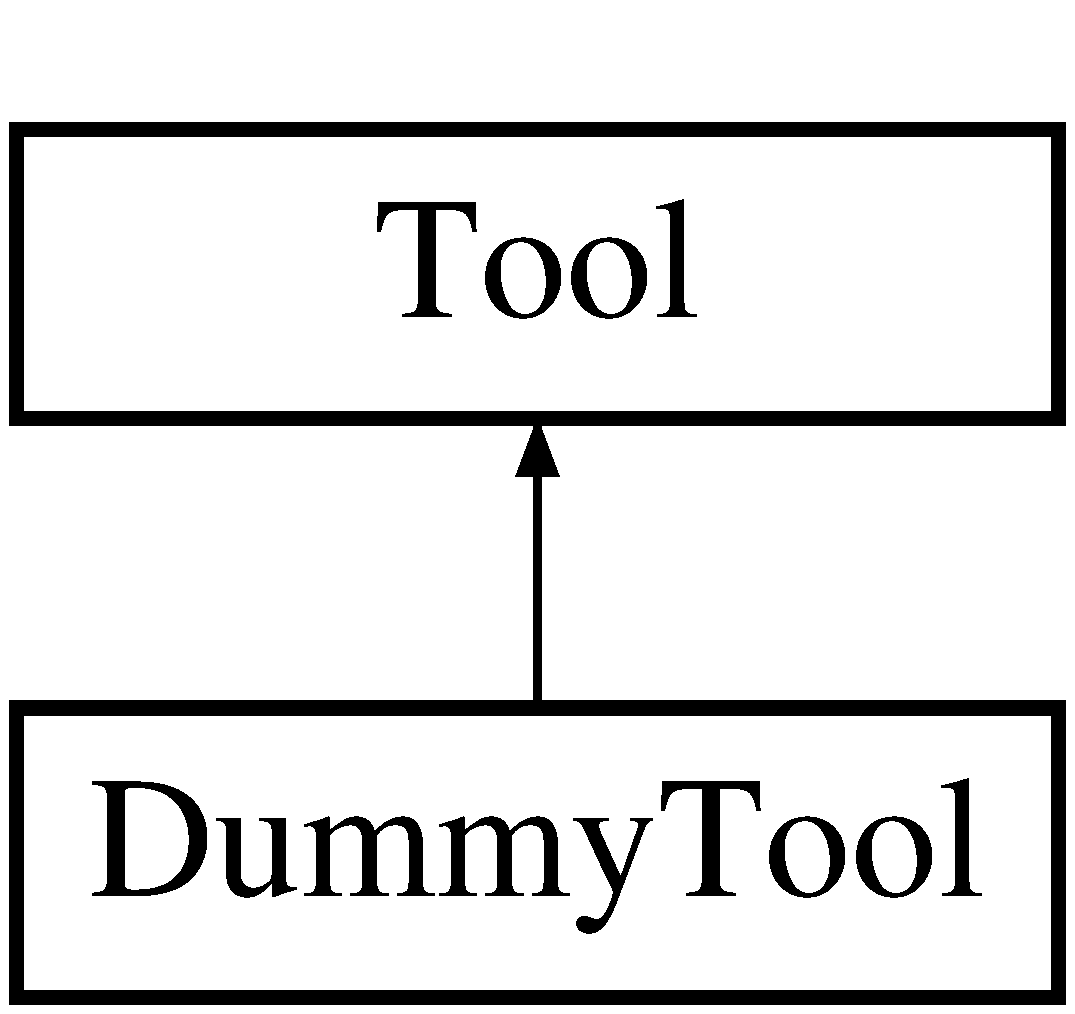
\includegraphics[height=2.000000cm]{classDummyTool}
\end{center}
\end{figure}
\subsection*{Public Member Functions}
\begin{DoxyCompactItemize}
\item 
\hypertarget{classDummyTool_a33914471b4de346168aa92b5febb6f9c}{\hyperlink{classDummyTool_a33914471b4de346168aa92b5febb6f9c}{Dummy\-Tool} ()}\label{classDummyTool_a33914471b4de346168aa92b5febb6f9c}

\begin{DoxyCompactList}\small\item\em Constructor. \end{DoxyCompactList}\item 
\hypertarget{classDummyTool_a0d9cd781681a06ee3cf0cd1e7bb770a8}{bool \hyperlink{classDummyTool_a0d9cd781681a06ee3cf0cd1e7bb770a8}{Initialise} (std\-::string configfile, \hyperlink{classDataModel}{Data\-Model} \&data)}\label{classDummyTool_a0d9cd781681a06ee3cf0cd1e7bb770a8}

\begin{DoxyCompactList}\small\item\em Assigns verbosity from config file and creates a log message. \end{DoxyCompactList}\item 
\hypertarget{classDummyTool_ac107b31f1785c1cc803e0e65be548047}{bool \hyperlink{classDummyTool_ac107b31f1785c1cc803e0e65be548047}{Execute} ()}\label{classDummyTool_ac107b31f1785c1cc803e0e65be548047}

\begin{DoxyCompactList}\small\item\em Creates a log message. \end{DoxyCompactList}\item 
\hypertarget{classDummyTool_aacb5d0b9906a27c2b4bba4aae9bc093a}{bool \hyperlink{classDummyTool_aacb5d0b9906a27c2b4bba4aae9bc093a}{Finalise} ()}\label{classDummyTool_aacb5d0b9906a27c2b4bba4aae9bc093a}

\begin{DoxyCompactList}\small\item\em Does nothing. \end{DoxyCompactList}\end{DoxyCompactItemize}


\subsection{Detailed Description}
This is a simple dummy Tool designed to show operation of a Tool. It also provides a default Tool for the Default Tool\-Chain.

\begin{DoxyParagraph}{Author\-:}
B.\-Richards 
\end{DoxyParagraph}
\begin{DoxyParagraph}{Date\-:}
2019/05/28 10\-:44\-:00 
\end{DoxyParagraph}
Contact\-: \href{mailto:b.richards@qmul.ac.uk}{\tt b.\-richards@qmul.\-ac.\-uk} 

The documentation for this class was generated from the following files\-:\begin{DoxyCompactItemize}
\item 
User\-Tools/\-Dummy\-Tool/Dummy\-Tool.\-h\item 
User\-Tools/\-Dummy\-Tool/Dummy\-Tool.\-cpp\end{DoxyCompactItemize}

\hypertarget{classMyTool}{}\doxysection{My\+Tool Class Reference}
\label{classMyTool}\index{MyTool@{MyTool}}


{\ttfamily \#include $<$My\+Tool.\+h$>$}

Inheritance diagram for My\+Tool\+:\begin{figure}[H]
\begin{center}
\leavevmode
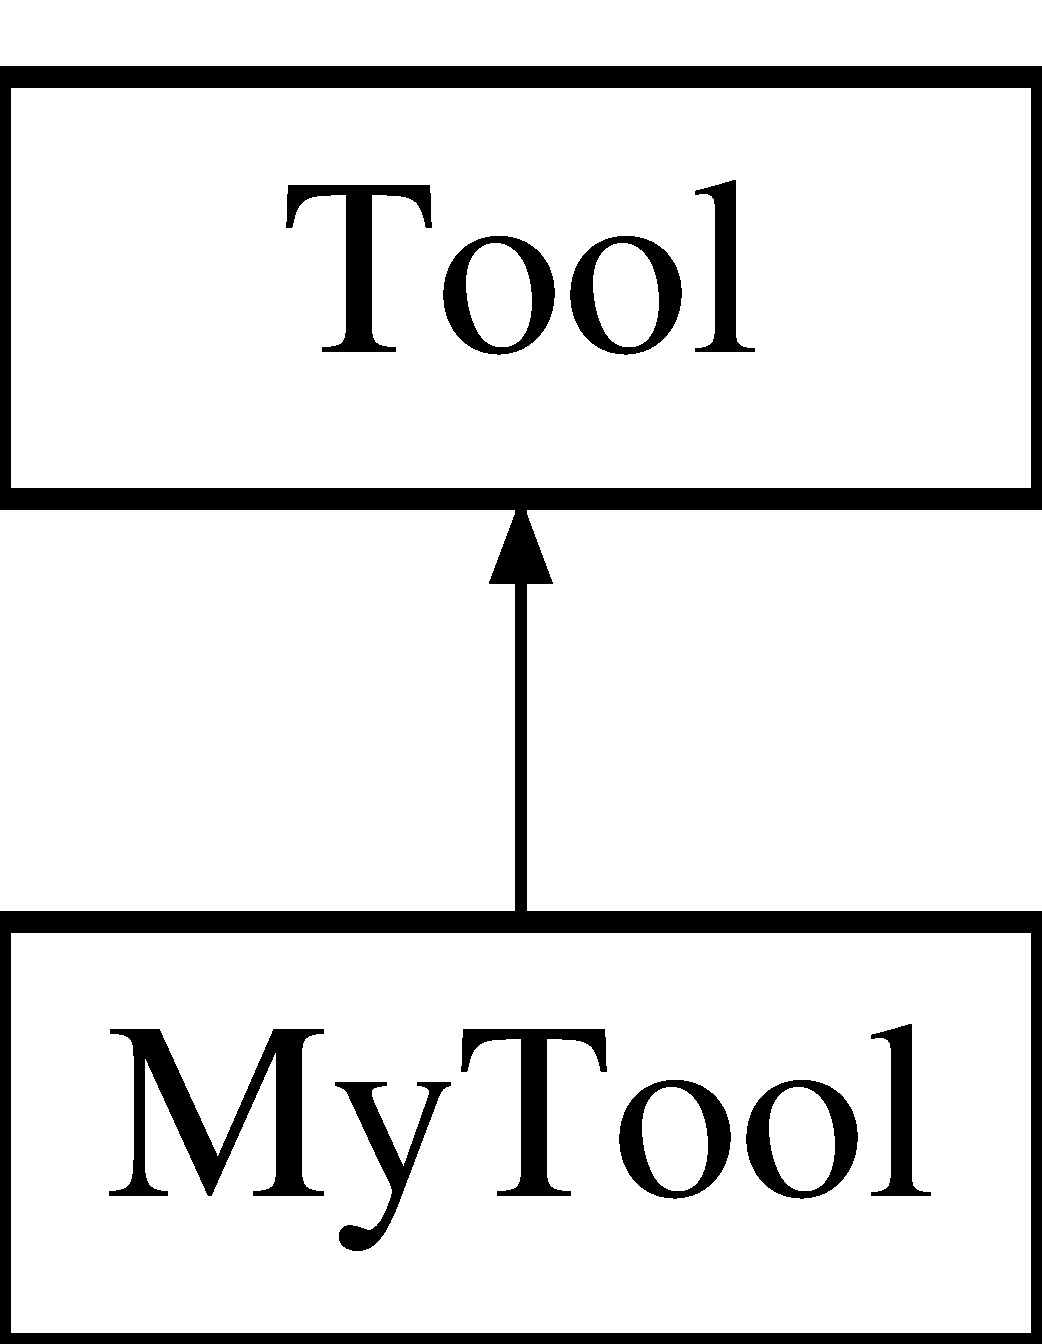
\includegraphics[height=2.000000cm]{classMyTool}
\end{center}
\end{figure}
\doxysubsection*{Public Member Functions}
\begin{DoxyCompactItemize}
\item 
\mbox{\Hypertarget{classMyTool_ad85b796bdd675ae22e69cf40fe7b6314}\label{classMyTool_ad85b796bdd675ae22e69cf40fe7b6314}} 
\mbox{\hyperlink{classMyTool_ad85b796bdd675ae22e69cf40fe7b6314}{My\+Tool}} ()
\begin{DoxyCompactList}\small\item\em Simple constructor. \end{DoxyCompactList}\item 
bool \mbox{\hyperlink{classMyTool_a3bf60061195a18542c4cfb2916b9dad9}{Initialise}} (std\+::string configfile, \mbox{\hyperlink{classDataModel}{Data\+Model}} \&data)
\begin{DoxyCompactList}\small\item\em Initialise Function for setting up Tool resorces. \end{DoxyCompactList}\item 
\mbox{\Hypertarget{classMyTool_a0a58122023af90b9200d0e71e89cfb36}\label{classMyTool_a0a58122023af90b9200d0e71e89cfb36}} 
bool \mbox{\hyperlink{classMyTool_a0a58122023af90b9200d0e71e89cfb36}{Execute}} ()
\begin{DoxyCompactList}\small\item\em Executre function used to perform Tool perpose. \end{DoxyCompactList}\item 
\mbox{\Hypertarget{classMyTool_a060ec6356451aa335d0de41093c9992f}\label{classMyTool_a060ec6356451aa335d0de41093c9992f}} 
bool \mbox{\hyperlink{classMyTool_a060ec6356451aa335d0de41093c9992f}{Finalise}} ()
\begin{DoxyCompactList}\small\item\em Finalise funciton used to clean up resorces. \end{DoxyCompactList}\end{DoxyCompactItemize}


\doxysubsection{Detailed Description}
This is a balnk template for a Tool used by the script to generate a new custom tool. Please fill out the descripton and author information.

\begin{DoxyParagraph}{Author}
B.\+Richards 
\end{DoxyParagraph}
\begin{DoxyParagraph}{Date}
2019/05/28 10\+:44\+:00 
\end{DoxyParagraph}


\doxysubsection{Member Function Documentation}
\mbox{\Hypertarget{classMyTool_a3bf60061195a18542c4cfb2916b9dad9}\label{classMyTool_a3bf60061195a18542c4cfb2916b9dad9}} 
\index{MyTool@{MyTool}!Initialise@{Initialise}}
\index{Initialise@{Initialise}!MyTool@{MyTool}}
\doxysubsubsection{\texorpdfstring{Initialise()}{Initialise()}}
{\footnotesize\ttfamily bool My\+Tool\+::\+Initialise (\begin{DoxyParamCaption}\item[{std\+::string}]{configfile,  }\item[{\mbox{\hyperlink{classDataModel}{Data\+Model}} \&}]{data }\end{DoxyParamCaption})}



Initialise Function for setting up Tool resorces. 


\begin{DoxyParams}{Parameters}
{\em configfile} & The path and name of the dynamic configuration file to read in.\\
\hline
{\em data} & A reference to the transient data class used to pass information between Tools. \\
\hline
\end{DoxyParams}


The documentation for this class was generated from the following files\+:\begin{DoxyCompactItemize}
\item 
User\+Tools/template/My\+Tool.\+h\item 
User\+Tools/template/My\+Tool.\+cpp\end{DoxyCompactItemize}

\hypertarget{classMyToolDynamicMultiThread}{\section{My\-Tool\-Dynamic\-Multi\-Thread Class Reference}
\label{classMyToolDynamicMultiThread}\index{My\-Tool\-Dynamic\-Multi\-Thread@{My\-Tool\-Dynamic\-Multi\-Thread}}
}


{\ttfamily \#include $<$My\-Tool\-Dynamic\-Multi\-Thread.\-h$>$}

Inheritance diagram for My\-Tool\-Dynamic\-Multi\-Thread\-:\begin{figure}[H]
\begin{center}
\leavevmode
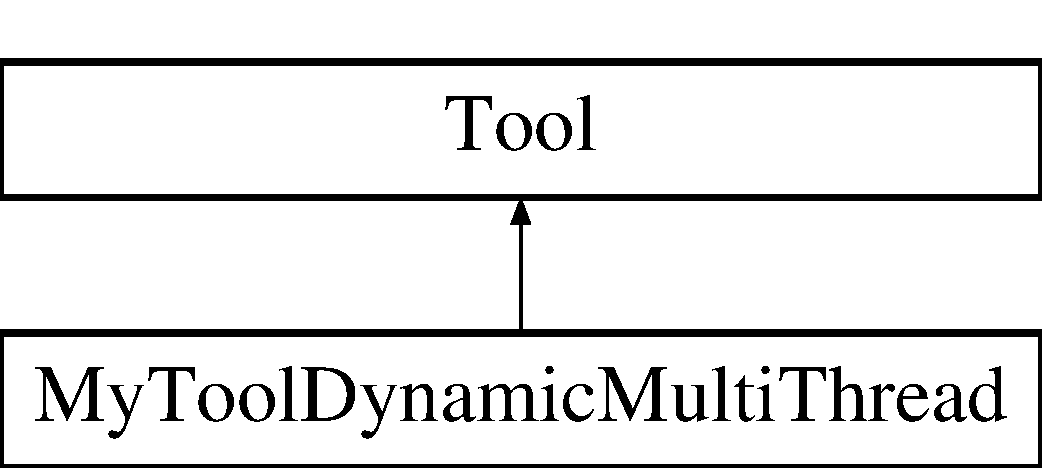
\includegraphics[height=2.000000cm]{classMyToolDynamicMultiThread}
\end{center}
\end{figure}
\subsection*{Public Member Functions}
\begin{DoxyCompactItemize}
\item 
\hypertarget{classMyToolDynamicMultiThread_a5eec7239400c507754ba6218b3eb8d4a}{\hyperlink{classMyToolDynamicMultiThread_a5eec7239400c507754ba6218b3eb8d4a}{My\-Tool\-Dynamic\-Multi\-Thread} ()}\label{classMyToolDynamicMultiThread_a5eec7239400c507754ba6218b3eb8d4a}

\begin{DoxyCompactList}\small\item\em Simple constructor. \end{DoxyCompactList}\item 
bool \hyperlink{classMyToolDynamicMultiThread_ac082408d85bc3e76214e55d4f62de0da}{Initialise} (std\-::string configfile, \hyperlink{classDataModel}{Data\-Model} \&data)
\begin{DoxyCompactList}\small\item\em Initialise Function for setting up Tool resorces. \end{DoxyCompactList}\item 
\hypertarget{classMyToolDynamicMultiThread_aec2f9af9495520d74bb154d626a94a63}{bool \hyperlink{classMyToolDynamicMultiThread_aec2f9af9495520d74bb154d626a94a63}{Execute} ()}\label{classMyToolDynamicMultiThread_aec2f9af9495520d74bb154d626a94a63}

\begin{DoxyCompactList}\small\item\em Executre function used to perform Tool perpose. \end{DoxyCompactList}\item 
\hypertarget{classMyToolDynamicMultiThread_ab70e77b0fd90e50c5103ccfa0bfd6485}{bool \hyperlink{classMyToolDynamicMultiThread_ab70e77b0fd90e50c5103ccfa0bfd6485}{Finalise} ()}\label{classMyToolDynamicMultiThread_ab70e77b0fd90e50c5103ccfa0bfd6485}

\begin{DoxyCompactList}\small\item\em Finalise funciton used to clean up resorces. \end{DoxyCompactList}\end{DoxyCompactItemize}


\subsection{Detailed Description}
This is a template for a Tool that dynamically more or less threads, such that there is always 1 available thread.\-This can therefore be used to scale to your worklaod, however be carefull when using more than one of these tools and to apply upperlimits if necessary both locally within this tool and globally so that more threads than is practical are created causing massive inefficency. Please fill out the descripton and author information.

\begin{DoxyParagraph}{Author\-:}
B.\-Richards 
\end{DoxyParagraph}
\begin{DoxyParagraph}{Date\-:}
2019/05/28 10\-:44\-:00 
\end{DoxyParagraph}
Contact\-: \href{mailto:b.richards@qmul.ac.uk}{\tt b.\-richards@qmul.\-ac.\-uk} 

\subsection{Member Function Documentation}
\hypertarget{classMyToolDynamicMultiThread_ac082408d85bc3e76214e55d4f62de0da}{\index{My\-Tool\-Dynamic\-Multi\-Thread@{My\-Tool\-Dynamic\-Multi\-Thread}!Initialise@{Initialise}}
\index{Initialise@{Initialise}!MyToolDynamicMultiThread@{My\-Tool\-Dynamic\-Multi\-Thread}}
\subsubsection[{Initialise}]{\setlength{\rightskip}{0pt plus 5cm}bool My\-Tool\-Dynamic\-Multi\-Thread\-::\-Initialise (
\begin{DoxyParamCaption}
\item[{std\-::string}]{configfile, }
\item[{{\bf Data\-Model} \&}]{data}
\end{DoxyParamCaption}
)}}\label{classMyToolDynamicMultiThread_ac082408d85bc3e76214e55d4f62de0da}


Initialise Function for setting up Tool resorces. 


\begin{DoxyParams}{Parameters}
{\em configfile} & The path and name of the dynamic configuration file to read in. \\
\hline
{\em data} & A reference to the transient data class used to pass information between Tools. \\
\hline
\end{DoxyParams}


The documentation for this class was generated from the following files\-:\begin{DoxyCompactItemize}
\item 
User\-Tools/template/My\-Tool\-Dynamic\-Multi\-Thread.\-h\item 
User\-Tools/template/My\-Tool\-Dynamic\-Multi\-Thread.\-cpp\end{DoxyCompactItemize}

\hypertarget{structMyToolDynamicMultiThread__args}{}\doxysection{My\+Tool\+Dynamic\+Multi\+Thread\+\_\+args Struct Reference}
\label{structMyToolDynamicMultiThread__args}\index{MyToolDynamicMultiThread\_args@{MyToolDynamicMultiThread\_args}}


{\ttfamily \#include $<$My\+Tool\+Dynamic\+Multi\+Thread.\+h$>$}

Inheritance diagram for My\+Tool\+Dynamic\+Multi\+Thread\+\_\+args\+:\begin{figure}[H]
\begin{center}
\leavevmode
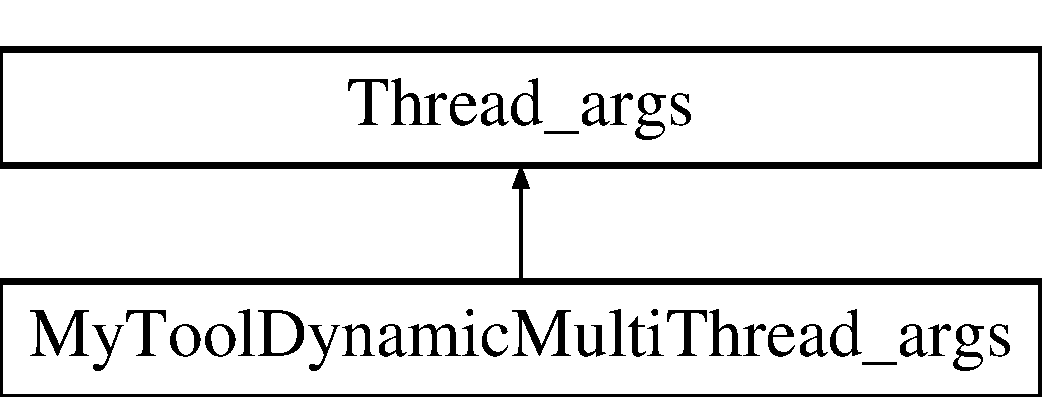
\includegraphics[height=2.000000cm]{structMyToolDynamicMultiThread__args}
\end{center}
\end{figure}
\doxysubsection*{Public Attributes}
\begin{DoxyCompactItemize}
\item 
\mbox{\Hypertarget{structMyToolDynamicMultiThread__args_a2d4b96b18b6e91a4244473e9e28c881b}\label{structMyToolDynamicMultiThread__args_a2d4b96b18b6e91a4244473e9e28c881b}} 
bool {\bfseries busy}
\item 
\mbox{\Hypertarget{structMyToolDynamicMultiThread__args_a4fe59813f550a1c10a2ab6527c580a23}\label{structMyToolDynamicMultiThread__args_a4fe59813f550a1c10a2ab6527c580a23}} 
std\+::string {\bfseries message}
\end{DoxyCompactItemize}
\doxysubsection*{Additional Inherited Members}


\doxysubsection{Detailed Description}
This is a struct to place data you want your thread to acess or exchange with it. The idea is the datainside is only used by the threa\textbackslash{} d and so will be thread safe

\begin{DoxyParagraph}{Author}
B.\+Richards 
\end{DoxyParagraph}
\begin{DoxyParagraph}{Date}
2019/05/28 10\+:44\+:00 
\end{DoxyParagraph}


The documentation for this struct was generated from the following files\+:\begin{DoxyCompactItemize}
\item 
User\+Tools/template/My\+Tool\+Dynamic\+Multi\+Thread.\+h\item 
User\+Tools/template/My\+Tool\+Dynamic\+Multi\+Thread.\+cpp\end{DoxyCompactItemize}

\hypertarget{classMyToolMultiThread}{}\doxysection{My\+Tool\+Multi\+Thread Class Reference}
\label{classMyToolMultiThread}\index{MyToolMultiThread@{MyToolMultiThread}}


{\ttfamily \#include $<$My\+Tool\+Multi\+Thread.\+h$>$}

Inheritance diagram for My\+Tool\+Multi\+Thread\+:\begin{figure}[H]
\begin{center}
\leavevmode
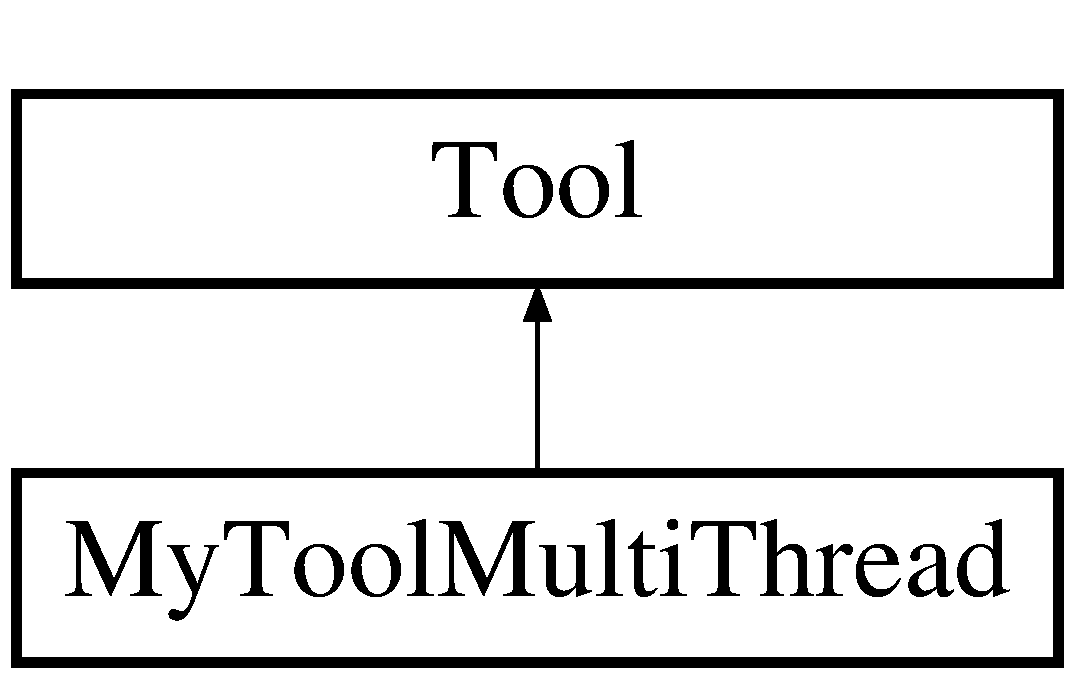
\includegraphics[height=2.000000cm]{classMyToolMultiThread}
\end{center}
\end{figure}
\doxysubsection*{Public Member Functions}
\begin{DoxyCompactItemize}
\item 
\mbox{\Hypertarget{classMyToolMultiThread_ac24f005c6da9c552871f6ff2672cf7f1}\label{classMyToolMultiThread_ac24f005c6da9c552871f6ff2672cf7f1}} 
\mbox{\hyperlink{classMyToolMultiThread_ac24f005c6da9c552871f6ff2672cf7f1}{My\+Tool\+Multi\+Thread}} ()
\begin{DoxyCompactList}\small\item\em Simple constructor. \end{DoxyCompactList}\item 
bool \mbox{\hyperlink{classMyToolMultiThread_a19dc55079a7b2da02ad9addd565b8e80}{Initialise}} (std\+::string configfile, \mbox{\hyperlink{classDataModel}{Data\+Model}} \&data)
\begin{DoxyCompactList}\small\item\em Initialise Function for setting up Tool resorces. \end{DoxyCompactList}\item 
\mbox{\Hypertarget{classMyToolMultiThread_a9cd7c894fc4797b2d81e12e25eb5beec}\label{classMyToolMultiThread_a9cd7c894fc4797b2d81e12e25eb5beec}} 
bool \mbox{\hyperlink{classMyToolMultiThread_a9cd7c894fc4797b2d81e12e25eb5beec}{Execute}} ()
\begin{DoxyCompactList}\small\item\em Executre function used to perform Tool perpose. \end{DoxyCompactList}\item 
\mbox{\Hypertarget{classMyToolMultiThread_a8f25561dc6a5daf8f4db85afecbb2c38}\label{classMyToolMultiThread_a8f25561dc6a5daf8f4db85afecbb2c38}} 
bool \mbox{\hyperlink{classMyToolMultiThread_a8f25561dc6a5daf8f4db85afecbb2c38}{Finalise}} ()
\begin{DoxyCompactList}\small\item\em Finalise funciton used to clean up resorces. \end{DoxyCompactList}\end{DoxyCompactItemize}


\doxysubsection{Detailed Description}
This is a template for a Tool That employs mulitple threads. Please fill out the descripton and author information.

\begin{DoxyParagraph}{Author}
B.\+Richards 
\end{DoxyParagraph}
\begin{DoxyParagraph}{Date}
2019/05/28 10\+:44\+:00 
\end{DoxyParagraph}


\doxysubsection{Member Function Documentation}
\mbox{\Hypertarget{classMyToolMultiThread_a19dc55079a7b2da02ad9addd565b8e80}\label{classMyToolMultiThread_a19dc55079a7b2da02ad9addd565b8e80}} 
\index{MyToolMultiThread@{MyToolMultiThread}!Initialise@{Initialise}}
\index{Initialise@{Initialise}!MyToolMultiThread@{MyToolMultiThread}}
\doxysubsubsection{\texorpdfstring{Initialise()}{Initialise()}}
{\footnotesize\ttfamily bool My\+Tool\+Multi\+Thread\+::\+Initialise (\begin{DoxyParamCaption}\item[{std\+::string}]{configfile,  }\item[{\mbox{\hyperlink{classDataModel}{Data\+Model}} \&}]{data }\end{DoxyParamCaption})}



Initialise Function for setting up Tool resorces. 


\begin{DoxyParams}{Parameters}
{\em configfile} & The path and name of the dynamic configuration file to read in.\\
\hline
{\em data} & A reference to the transient data class used to pass information between Tools. \\
\hline
\end{DoxyParams}


The documentation for this class was generated from the following files\+:\begin{DoxyCompactItemize}
\item 
User\+Tools/template/My\+Tool\+Multi\+Thread.\+h\item 
User\+Tools/template/My\+Tool\+Multi\+Thread.\+cpp\end{DoxyCompactItemize}

\hypertarget{structMyToolMultiThread__args}{}\doxysection{My\+Tool\+Multi\+Thread\+\_\+args Struct Reference}
\label{structMyToolMultiThread__args}\index{MyToolMultiThread\_args@{MyToolMultiThread\_args}}


{\ttfamily \#include $<$My\+Tool\+Multi\+Thread.\+h$>$}

Inheritance diagram for My\+Tool\+Multi\+Thread\+\_\+args\+:\begin{figure}[H]
\begin{center}
\leavevmode
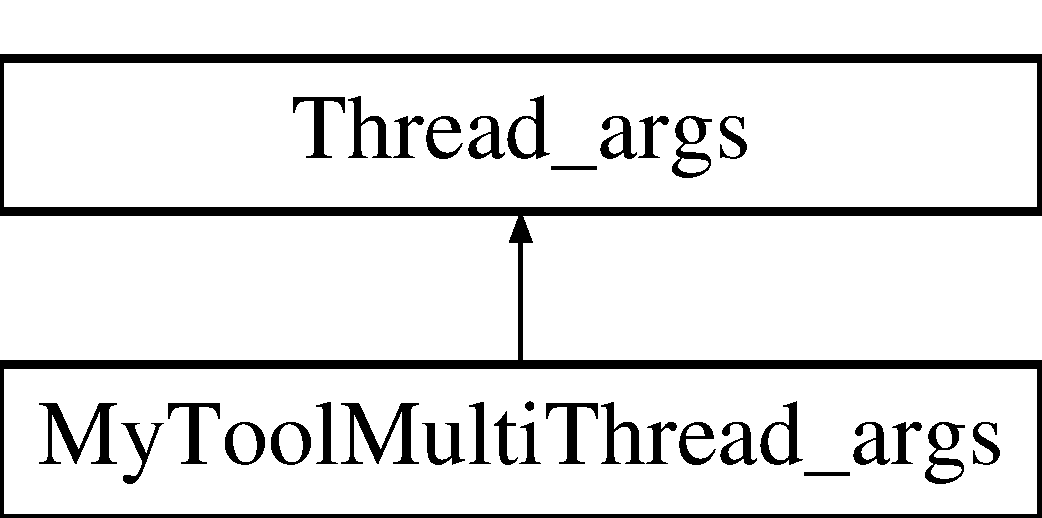
\includegraphics[height=2.000000cm]{structMyToolMultiThread__args}
\end{center}
\end{figure}
\doxysubsection*{Public Attributes}
\begin{DoxyCompactItemize}
\item 
\mbox{\Hypertarget{structMyToolMultiThread__args_a25e00c4f60078d432869910f475fff9b}\label{structMyToolMultiThread__args_a25e00c4f60078d432869910f475fff9b}} 
bool {\bfseries busy}
\item 
\mbox{\Hypertarget{structMyToolMultiThread__args_a05324a4ea6b7c87b2cc09473ab9027f5}\label{structMyToolMultiThread__args_a05324a4ea6b7c87b2cc09473ab9027f5}} 
std\+::string {\bfseries message}
\end{DoxyCompactItemize}
\doxysubsection*{Additional Inherited Members}


\doxysubsection{Detailed Description}
This is a struct to place data you want your thread to acess or exchange with it. The idea is the datainside is only used by the thread and so will be thread safe

\begin{DoxyParagraph}{Author}
B.\+Richards 
\end{DoxyParagraph}
\begin{DoxyParagraph}{Date}
2019/05/28 10\+:44\+:00 
\end{DoxyParagraph}


The documentation for this struct was generated from the following files\+:\begin{DoxyCompactItemize}
\item 
User\+Tools/template/My\+Tool\+Multi\+Thread.\+h\item 
User\+Tools/template/My\+Tool\+Multi\+Thread.\+cpp\end{DoxyCompactItemize}

\hypertarget{classMyToolThread}{\section{My\-Tool\-Thread Class Reference}
\label{classMyToolThread}\index{My\-Tool\-Thread@{My\-Tool\-Thread}}
}


{\ttfamily \#include $<$My\-Tool\-Thread.\-h$>$}

Inheritance diagram for My\-Tool\-Thread\-:\begin{figure}[H]
\begin{center}
\leavevmode
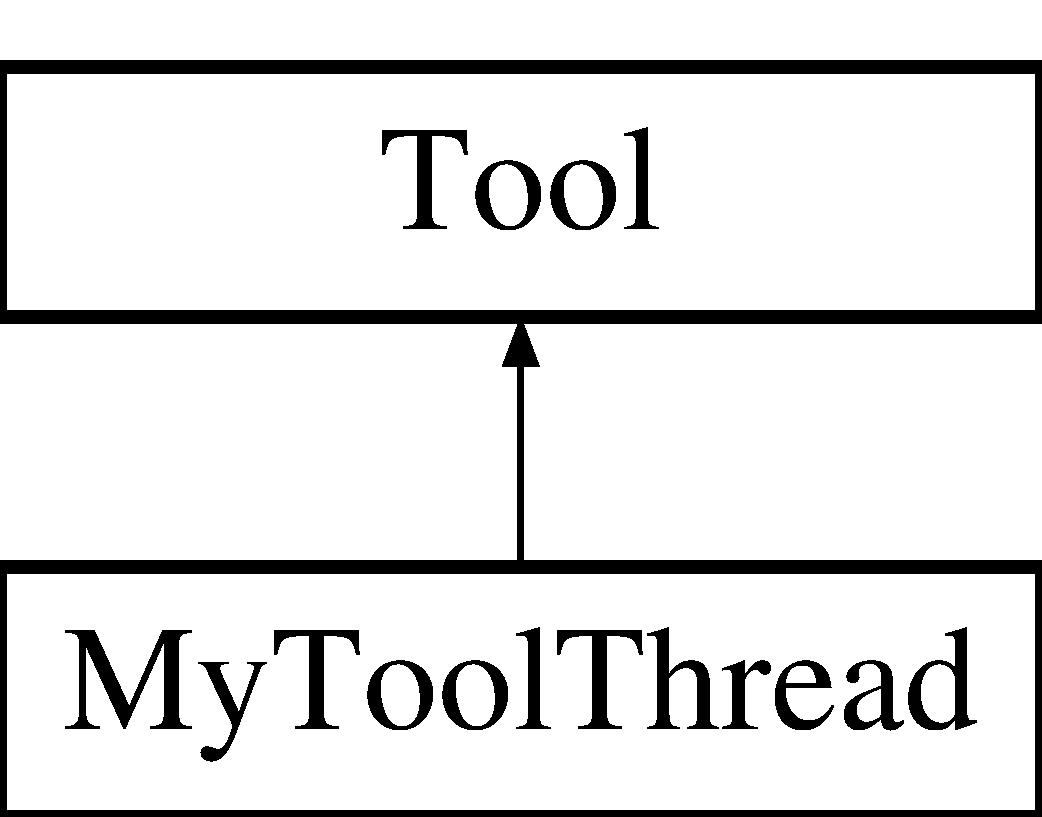
\includegraphics[height=2.000000cm]{classMyToolThread}
\end{center}
\end{figure}
\subsection*{Public Member Functions}
\begin{DoxyCompactItemize}
\item 
\hypertarget{classMyToolThread_a66c6fc304a8d62436281598d988dd845}{\hyperlink{classMyToolThread_a66c6fc304a8d62436281598d988dd845}{My\-Tool\-Thread} ()}\label{classMyToolThread_a66c6fc304a8d62436281598d988dd845}

\begin{DoxyCompactList}\small\item\em Simple constructor. \end{DoxyCompactList}\item 
bool \hyperlink{classMyToolThread_adc7ab1ab74fc1564f07e52e63383d679}{Initialise} (std\-::string configfile, \hyperlink{classDataModel}{Data\-Model} \&data)
\begin{DoxyCompactList}\small\item\em Initialise Function for setting up Tool resorces. \end{DoxyCompactList}\item 
\hypertarget{classMyToolThread_a9b582cd202d5578682d57d973988df3c}{bool \hyperlink{classMyToolThread_a9b582cd202d5578682d57d973988df3c}{Execute} ()}\label{classMyToolThread_a9b582cd202d5578682d57d973988df3c}

\begin{DoxyCompactList}\small\item\em Executre function used to perform Tool perpose. \end{DoxyCompactList}\item 
\hypertarget{classMyToolThread_aa51e385684efcb19f1c039b96653070e}{bool \hyperlink{classMyToolThread_aa51e385684efcb19f1c039b96653070e}{Finalise} ()}\label{classMyToolThread_aa51e385684efcb19f1c039b96653070e}

\begin{DoxyCompactList}\small\item\em Finalise funciton used to clean up resorces. \end{DoxyCompactList}\end{DoxyCompactItemize}


\subsection{Detailed Description}
This is a template for a Tool that produces a single thread that can be assigned a function seperate to the main thread. Please fill out the descripton and author information.

\begin{DoxyParagraph}{Author\-:}
B.\-Richards 
\end{DoxyParagraph}
\begin{DoxyParagraph}{Date\-:}
2019/05/28 10\-:44\-:00 
\end{DoxyParagraph}
Contact\-: \href{mailto:b.richards@qmul.ac.uk}{\tt b.\-richards@qmul.\-ac.\-uk} 

\subsection{Member Function Documentation}
\hypertarget{classMyToolThread_adc7ab1ab74fc1564f07e52e63383d679}{\index{My\-Tool\-Thread@{My\-Tool\-Thread}!Initialise@{Initialise}}
\index{Initialise@{Initialise}!MyToolThread@{My\-Tool\-Thread}}
\subsubsection[{Initialise}]{\setlength{\rightskip}{0pt plus 5cm}bool My\-Tool\-Thread\-::\-Initialise (
\begin{DoxyParamCaption}
\item[{std\-::string}]{configfile, }
\item[{{\bf Data\-Model} \&}]{data}
\end{DoxyParamCaption}
)}}\label{classMyToolThread_adc7ab1ab74fc1564f07e52e63383d679}


Initialise Function for setting up Tool resorces. 


\begin{DoxyParams}{Parameters}
{\em configfile} & The path and name of the dynamic configuration file to read in. \\
\hline
{\em data} & A reference to the transient data class used to pass information between Tools. \\
\hline
\end{DoxyParams}


The documentation for this class was generated from the following files\-:\begin{DoxyCompactItemize}
\item 
User\-Tools/template/My\-Tool\-Thread.\-h\item 
User\-Tools/template/My\-Tool\-Thread.\-cpp\end{DoxyCompactItemize}

\hypertarget{structMyToolThread__args}{}\doxysection{My\+Tool\+Thread\+\_\+args Struct Reference}
\label{structMyToolThread__args}\index{MyToolThread\_args@{MyToolThread\_args}}
Inheritance diagram for My\+Tool\+Thread\+\_\+args\+:\begin{figure}[H]
\begin{center}
\leavevmode
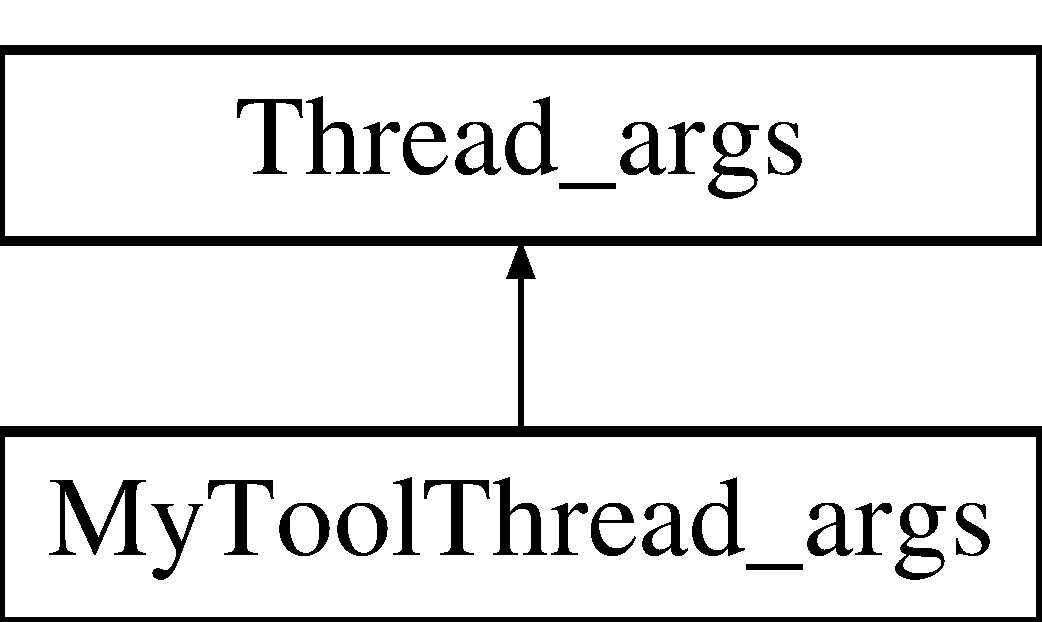
\includegraphics[height=2.000000cm]{structMyToolThread__args}
\end{center}
\end{figure}
\doxysubsection*{Additional Inherited Members}


The documentation for this struct was generated from the following files\+:\begin{DoxyCompactItemize}
\item 
User\+Tools/template/My\+Tool\+Thread.\+h\item 
User\+Tools/template/My\+Tool\+Thread.\+cpp\end{DoxyCompactItemize}

\hypertarget{structMyToolThread__args__args}{\section{My\-Tool\-Thread\-\_\-args\-\_\-args Struct Reference}
\label{structMyToolThread__args__args}\index{My\-Tool\-Thread\-\_\-args\-\_\-args@{My\-Tool\-Thread\-\_\-args\-\_\-args}}
}


{\ttfamily \#include $<$My\-Tool\-Thread.\-h$>$}



\subsection{Detailed Description}
This is a struct to place data you want your thread to access or exchange with it. The idea is the datainside is only used by the threa and so will be thread safe

\begin{DoxyParagraph}{Author\-:}
B.\-Richards 
\end{DoxyParagraph}
\begin{DoxyParagraph}{Date\-:}
2019/05/28 10\-:44\-:00 
\end{DoxyParagraph}
Contact\-: \href{mailto:b.richards@qmul.ac.uk}{\tt b.\-richards@qmul.\-ac.\-uk} 

The documentation for this struct was generated from the following file\-:\begin{DoxyCompactItemize}
\item 
User\-Tools/template/My\-Tool\-Thread.\-h\end{DoxyCompactItemize}

\hypertarget{structThread__args}{}\doxysection{Thread\+\_\+args Struct Reference}
\label{structThread__args}\index{Thread\_args@{Thread\_args}}
Inheritance diagram for Thread\+\_\+args\+:\begin{figure}[H]
\begin{center}
\leavevmode
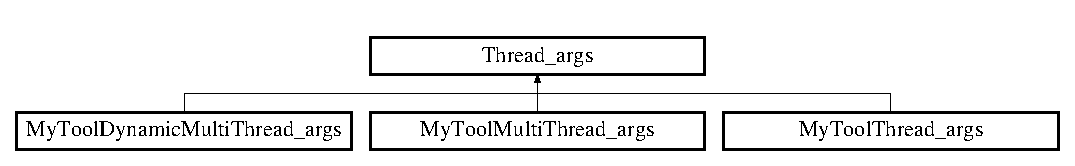
\includegraphics[height=1.600000cm]{structThread__args}
\end{center}
\end{figure}
\doxysubsection*{Public Member Functions}
\begin{DoxyCompactItemize}
\item 
\mbox{\hyperlink{structThread__args_a399b672e0f4f137fe52c141bd8c38eb1}{Thread\+\_\+args}} ()
\item 
virtual \mbox{\hyperlink{structThread__args_ad786e0c55b4e44bc04d9ba3b813bace1}{$\sim$\+Thread\+\_\+args}} ()
\end{DoxyCompactItemize}
\doxysubsection*{Public Attributes}
\begin{DoxyCompactItemize}
\item 
\mbox{\Hypertarget{structThread__args_a594f831be7ce66015a7606e023b24cf4}\label{structThread__args_a594f831be7ce66015a7606e023b24cf4}} 
std\+::string \mbox{\hyperlink{structThread__args_a594f831be7ce66015a7606e023b24cf4}{Thread\+Name}}
\begin{DoxyCompactList}\small\item\em name of thread (deffined at creation) \end{DoxyCompactList}\item 
\mbox{\Hypertarget{structThread__args_ad5950e8a9a345f012c6b11a8d9dc7cc2}\label{structThread__args_ad5950e8a9a345f012c6b11a8d9dc7cc2}} 
void($\ast$ \mbox{\hyperlink{structThread__args_ad5950e8a9a345f012c6b11a8d9dc7cc2}{func}} )(\mbox{\hyperlink{structThread__args}{Thread\+\_\+args}} $\ast$)
\begin{DoxyCompactList}\small\item\em function pointer to thread with args \end{DoxyCompactList}\item 
\mbox{\Hypertarget{structThread__args_a4f71beb11e75d05269fc63ca7c19a8a9}\label{structThread__args_a4f71beb11e75d05269fc63ca7c19a8a9}} 
pthread\+\_\+t \mbox{\hyperlink{structThread__args_a4f71beb11e75d05269fc63ca7c19a8a9}{thread}}
\begin{DoxyCompactList}\small\item\em Simple constructor underlying thread that interface is built ontop of. \end{DoxyCompactList}\item 
\mbox{\Hypertarget{structThread__args_a9cb8f6b709c5687bf28531bf4d808c75}\label{structThread__args_a9cb8f6b709c5687bf28531bf4d808c75}} 
bool \mbox{\hyperlink{structThread__args_a9cb8f6b709c5687bf28531bf4d808c75}{running}}
\begin{DoxyCompactList}\small\item\em Bool flag to tell the thread to run (if not set thread goes into wait cycle. \end{DoxyCompactList}\item 
\mbox{\Hypertarget{structThread__args_a298b8c85c8598ecc557e2090d90a73c3}\label{structThread__args_a298b8c85c8598ecc557e2090d90a73c3}} 
bool \mbox{\hyperlink{structThread__args_a298b8c85c8598ecc557e2090d90a73c3}{kill}}
\begin{DoxyCompactList}\small\item\em Bool flay used to kill the thread. \end{DoxyCompactList}\end{DoxyCompactItemize}


\doxysubsection{Constructor \& Destructor Documentation}
\mbox{\Hypertarget{structThread__args_a399b672e0f4f137fe52c141bd8c38eb1}\label{structThread__args_a399b672e0f4f137fe52c141bd8c38eb1}} 
\index{Thread\_args@{Thread\_args}!Thread\_args@{Thread\_args}}
\index{Thread\_args@{Thread\_args}!Thread\_args@{Thread\_args}}
\doxysubsubsection{\texorpdfstring{Thread\_args()}{Thread\_args()}}
{\footnotesize\ttfamily Thread\+\_\+args\+::\+Thread\+\_\+args (\begin{DoxyParamCaption}{ }\end{DoxyParamCaption})\hspace{0.3cm}{\ttfamily [inline]}}

$<$ Simple constructor\mbox{\Hypertarget{structThread__args_ad786e0c55b4e44bc04d9ba3b813bace1}\label{structThread__args_ad786e0c55b4e44bc04d9ba3b813bace1}} 
\index{Thread\_args@{Thread\_args}!````~Thread\_args@{$\sim$Thread\_args}}
\index{````~Thread\_args@{$\sim$Thread\_args}!Thread\_args@{Thread\_args}}
\doxysubsubsection{\texorpdfstring{$\sim$Thread\_args()}{~Thread\_args()}}
{\footnotesize\ttfamily virtual Thread\+\_\+args\+::$\sim$\+Thread\+\_\+args (\begin{DoxyParamCaption}{ }\end{DoxyParamCaption})\hspace{0.3cm}{\ttfamily [inline]}, {\ttfamily [virtual]}}

$<$ virtual constructor

The documentation for this struct was generated from the following file\+:\begin{DoxyCompactItemize}
\item 
Data\+Model/Utilities.\+h\end{DoxyCompactItemize}

\hypertarget{classUtilities}{}\doxysection{Utilities Class Reference}
\label{classUtilities}\index{Utilities@{Utilities}}


{\ttfamily \#include $<$Utilities.\+h$>$}

Inheritance diagram for Utilities\+:\begin{figure}[H]
\begin{center}
\leavevmode
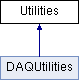
\includegraphics[height=2.000000cm]{classUtilities}
\end{center}
\end{figure}
\doxysubsection*{Public Member Functions}
\begin{DoxyCompactItemize}
\item 
\mbox{\Hypertarget{classUtilities_ab1676c9ce35cf347a73d16f1094e1271}\label{classUtilities_ab1676c9ce35cf347a73d16f1094e1271}} 
\mbox{\hyperlink{classUtilities_ab1676c9ce35cf347a73d16f1094e1271}{Utilities}} ()
\begin{DoxyCompactList}\small\item\em Simple constructor. \end{DoxyCompactList}\item 
\mbox{\Hypertarget{classUtilities_ae52d1dd16b34518b2ef4de01660cb8b2}\label{classUtilities_ae52d1dd16b34518b2ef4de01660cb8b2}} 
\mbox{\hyperlink{structThread__args}{Thread\+\_\+args}} $\ast$ \mbox{\hyperlink{classUtilities_ae52d1dd16b34518b2ef4de01660cb8b2}{Create\+Thread}} (std\+::string Thread\+Name, void($\ast$func)(\mbox{\hyperlink{structThread__args}{Thread\+\_\+args}} $\ast$), \mbox{\hyperlink{structThread__args}{Thread\+\_\+args}} $\ast$args)
\begin{DoxyCompactList}\small\item\em Create a thread with more complicated data exchange definned by arguments. \end{DoxyCompactList}\item 
\mbox{\Hypertarget{classUtilities_a6f1c1d53b9ce59bb26c56a3bebdbb255}\label{classUtilities_a6f1c1d53b9ce59bb26c56a3bebdbb255}} 
bool \mbox{\hyperlink{classUtilities_a6f1c1d53b9ce59bb26c56a3bebdbb255}{Kill\+Thread}} (\mbox{\hyperlink{structThread__args}{Thread\+\_\+args}} $\ast$\&args)
\begin{DoxyCompactList}\small\item\em Kill a thread assosiated to args. \end{DoxyCompactList}\item 
\mbox{\Hypertarget{classUtilities_a8c17a46ce33b0b647797f24bc859bd7a}\label{classUtilities_a8c17a46ce33b0b647797f24bc859bd7a}} 
bool \mbox{\hyperlink{classUtilities_a8c17a46ce33b0b647797f24bc859bd7a}{Kill\+Thread}} (std\+::string Thread\+Name)
\begin{DoxyCompactList}\small\item\em Kill a thread by name. \end{DoxyCompactList}\item 
\mbox{\Hypertarget{classUtilities_af4091a68d8a27a3b806d029cc9b2135e}\label{classUtilities_af4091a68d8a27a3b806d029cc9b2135e}} 
{\footnotesize template$<$typename T $>$ }\\bool \mbox{\hyperlink{classUtilities_af4091a68d8a27a3b806d029cc9b2135e}{Kill\+Thread}} (T $\ast$pointer)
\begin{DoxyCompactList}\small\item\em Kill a thread with args that inheirt form base \mbox{\hyperlink{structThread__args}{Thread\+\_\+args}}. \end{DoxyCompactList}\end{DoxyCompactItemize}
\doxysubsection*{Static Protected Member Functions}
\begin{DoxyCompactItemize}
\item 
\mbox{\Hypertarget{classUtilities_a29b7f99dcb44ddb9a519c3e441a7fa2b}\label{classUtilities_a29b7f99dcb44ddb9a519c3e441a7fa2b}} 
static void $\ast$ \mbox{\hyperlink{classUtilities_a29b7f99dcb44ddb9a519c3e441a7fa2b}{Thread}} (void $\ast$arg)
\begin{DoxyCompactList}\small\item\em Thread with args. \end{DoxyCompactList}\end{DoxyCompactItemize}
\doxysubsection*{Protected Attributes}
\begin{DoxyCompactItemize}
\item 
\mbox{\Hypertarget{classUtilities_a26ebd7308ea895452c4c1066dc5834e5}\label{classUtilities_a26ebd7308ea895452c4c1066dc5834e5}} 
std\+::map$<$ std\+::string, \mbox{\hyperlink{structThread__args}{Thread\+\_\+args}} $\ast$ $>$ \mbox{\hyperlink{classUtilities_a26ebd7308ea895452c4c1066dc5834e5}{Threads}}
\begin{DoxyCompactList}\small\item\em Map of threads managed by the utilities class. \end{DoxyCompactList}\end{DoxyCompactItemize}


\doxysubsection{Detailed Description}
This class can be instansiated in a Tool and provides some helpful threading, dynamic socket descovery and promotion functionality

\begin{DoxyParagraph}{Author}
B.\+Richards 
\end{DoxyParagraph}
\begin{DoxyParagraph}{Date}
2019/05/26 18\+:34\+:00 
\end{DoxyParagraph}


The documentation for this class was generated from the following files\+:\begin{DoxyCompactItemize}
\item 
Data\+Model/Utilities.\+h\item 
Data\+Model/Utilities.\+cpp\end{DoxyCompactItemize}

%--- End generated contents ---

% Index
\newpage
\phantomsection
\addcontentsline{toc}{part}{Index}
\printindex

\end{document}
